%% LyX 1.6.5 created this file.  For more info, see http://www.lyx.org/.
%% Do not edit unless you really know what you are doing.
\documentclass[12pt,oneside,ngerman]{scrbook}
\usepackage{ae,aecompl}
\usepackage[T1]{fontenc}
\usepackage[utf8]{inputenc}
\setcounter{secnumdepth}{3}
\setcounter{tocdepth}{3}
\usepackage{babel}

\usepackage{array}
\usepackage{longtable}
\usepackage{graphicx}
\usepackage[unicode=true, pdfusetitle,
 bookmarks=true,bookmarksnumbered=false,bookmarksopen=false,
 breaklinks=false,pdfborder={0 0 1},backref=false,colorlinks=false]
 {hyperref}

\makeatletter

%%%%%%%%%%%%%%%%%%%%%%%%%%%%%% LyX specific LaTeX commands.
%% Because html converters don't know tabularnewline
\providecommand{\tabularnewline}{\\}

\makeatother

\begin{document}

\title{Spezifikation aidGer}


\author{Buchgraber (2512046), Gildein (2513744), Pirrung (2526016)\\
Gruppe 10}

\maketitle
\tableofcontents{}


\chapter{Einleitung\label{cha:Einleitung}}


\section{Zweck\label{sec:Zweck}}

Diese Spezifikation dient als Grundlage für alle weitere Dokumente,
die im Rahmen dieses Softwarepraktikums entstehen. Sie enthält alle
wesentlichen Anforderungen an die Software und deren Schnittstellen.
Sie muss stets mit den anderen Dokumenten, insbesondere dem Entwurf
und der Codierung, konsistent gehalten werden. Die Spezifikation dient
den Teammitgliedern als Grundlage und Richtlinie bei der Entwicklung
des Systems.


\section{Leserkreis\label{sec:Leserkreis}}

Dieses Dokument ist für den folgenden Leserkreis bestimmt:
\begin{itemize}
\item Das gesamte Projektteam
\item Der Kunde
\item Die Betreuer des Softwarepraktikums
\item Der Gutachter des Spezifikationsreview
\item Die künftige Programmierer bzw. Verwalter dieses Projektes
\end{itemize}

\section{Einsatzbereich und Ziele\label{sec:Einsatzbereich-und-Ziele}}

In diesem Projekt soll das Hilfskraftverwaltungssystem ,,aidGer{}``
realisiert werden. Der ,,aidGer{}`` soll den Mitarbeitern der Abteilung
SE die tägliche Arbeit bei der Verwaltung der Hilfskraftbeschäftigungen
des Institutsverbund der Informatik erleichtern.\\
\\
Die neue Software dient hierbei grundsätzlich auch zur Erfassung
und Auswertung aller Vorgänge, die bei der Verwaltung von Hilfskräften
anfallen.\\
\\
Das Ziel ist es, mit ,,aidGer{}`` die jetzige Lösung ,,Hive{}``
zu ersetzen. Das Altsystem ,,Hive{}`` soll jedoch weiterhin einsetzbar
sein, um im Notfall oder bei ähnlichen Anlässen auf dieses zurückgreifen
zu können.


\section{Fachbegriffe und Abkürzungen}

Alle für dieses Projekt relevanten Fachbegriffe und Abkürzungen sind
in \ref{sec:Begriffslexikon} (im Anhang dieses Dokuments) aufgeführt.


\section{Aufbau dieses Dokuments}

Neben einer allgemeinen Beschreibung des Systems sollen die Anforderungen
an die Funktionen des Systems und die geforderten Qualitäten hinsichtlich
der Software dokumentiert werden. Im Anschluß hierzu wird auf die
Benutzeroberfläche und im nächsten Schritt auf die Anwendungsfälle
des Systems näher eingegangen. Das Dokument endet schließlich mit
einem angehängten Begriffslexikon.


\subsection{Konventionen}

In dieser Spezifikation werden die folgenden Konventionen zur Hervorhebung
von Begriffen verwendet:

%TODO: Issue 11


\chapter{Allgemeine Beschreibung\label{cha:Allgemeine-Beschreibung}}

In diesem Kapitel soll der ,,aidGer{}`` in seinen Grundzügen beschrieben
werden.


\section{Einbettung\label{sec:Einbettung}}

%TODO: Issue #5


Der ,,aidGer{}`` benötigt eine Schnittstelle zur verwendeten Datenbank.
Diese wird durch die Bibliothek AdoHive zur Verfügung gestellt.\\
\\
Zudem wird eine Verbindung mit dem bereits vorhandenen Ticket-System
benötigt. Diese Verbindung wird in Form einer Import- bzw. Exportschnitstelle
hergestellt, die jedoch in der ersten Software-Version nur vorgesehen
und beim Entwurf berücksichtigt wird. Eine spätere Implementierung
ist jedoch denkbar und in Zukunft vom Kunden auch ausdrücklich erwünscht.


\section{Grundlegende Funktionen\label{sec:Grundlegende-Funktionen}}

Der ,,aidGer{}`` soll dem Nutzer folgende Grundfunktionen bereitstellen:
\begin{itemize}
\item Verwaltung von Stammdaten: Veranstaltungen, Hilfskräfte, Finanzpläne,
Stundenlöhne
\item Anzeige von berechneten Daten: Budget aller Veranstaltungen (Budgetprüfung),
alle Beschäftigungen mit zugehörigem Vertrag, aggregierte Anzeigen
wie beispielsweise alle Vorgänge zu mehreren Hilfskräften oder Veranstaltungen
\item Buchung von Beschäftigungen mit Warnhinweisen bei bestimmten Ereignissen
\item Erfassung aller Vorgänge, die getätigt werden
\item Erleichterung des Controllings der Abrechnungen bzw. Auszugslisten
(Monatsauszug)
\item Generation möglichst vieler PDF-Berichte (Reporting)
\item Unterstützung bei der Benachrichtung mehrerer Hilfskräfte (Massenerfassung
von Vorgängen)
\item Tagesprotokoll über alle Vorgänge
\end{itemize}
Diese Funktionen sollen für alle Benutzer leicht erlernbar, effizient
und einfach in der Handhabung sein.


\section{Benutzerprofile\label{sec:Benutzerprofile}}

Die Software wird ausschließlich von den Mitarbeitern der Hilfskraftmittelverwaltung
des Institutsverbund für Informatik bedient. Daher sind diese die
einzige Benutzergruppe, die für die Software vorgesehen werden muss.
Sie haben ein fundiertes Wissen über alle Bereiche der Hilfskraftmittelverwaltung
und haben folglich alle Funktionen, die ,,aidGer{}`` bietet, bereits
im alten System oder auf Papier durchgeführt. Fundierte Kenntnisse
im Software Engineering können von den Mitarbeitern nicht angenommen
werden, da nicht klar ist, welche Abteilung die Hilfskraftmittelverwaltung
in ferner Zukunft übernimmt.


\section{Einschränkungen\label{sec:Einschr=0000E4nkungen}}

Die Vorgabe des Kunden hinsichtlich der Entwicklungsplattform ist
Java mit der SDK Version 6 als Programmiersprache und Swing als Oberflächenbibliothek.\\
\\
Zur Generierung von PDF-Berichten soll eine aktuelle Version der
iText Bibliothek eingesetzt werden. Um auf die Datenbank zuzugreifen,
soll die von Team AdoHive bereitgestellte AdoHive Bibliothek verwendet
werden. Andere externe Bibliotheken müssen durch den Betreuer explizit
genehmigt werden. Zur Anzeige von den generierten PDF-Berichten muss
der Anwender einen PDF-Betrachter installiert haben. Sollte das Programm
nicht in der Lage sein, den systemspezifischen PDF-Betrachter zu starten,
wird eine entsprechende Meldung dem Benutzer angezeigt.\\
\\
Zur Darstellung von Klassendiagrammen oder ähnlichen Diagrammen,
die während des Entwurfs entstehen, soll UML benutzt werden.\\
\\
Durch den Zeitplan ist ein Prozessmodel bereits vorgegeben.


\chapter{Anforderungen\label{cha:Anforderungen}}

In diesem Kapitel werden die Anforderungen an das System im Detail
beschrieben.


\section{Leistungsanforderungen\label{sec:Leistungsanforderungen}}

Da das Programm auf dem Server des Benutzers verwendet wird, darf
es andere Programme oder das Betriebssystem nicht behindern. Darüber
hinaus soll die Software alle Funktionen in möglichst geringer Zeit
($<$ 5 Sekunden) ausführen.


\section{Mengengerüst\label{sec:Mengenger=0000FCst}}

Folgende Kenngrößen sind für das System relevant:
\begin{itemize}
\item Das Programm ist eine Einzelplatzanwendung ohne Netzwerkfunktionalität
und wird daher stets von einem Anwender bedient
\item Das Programm wird in der Regel von maximal 3 verschiedenen Anwendern
bedient. Daher sind gleichzeitige Zugriffe auf die Datenbank von mehreren
Rechnern zu vernachlässigen
\item Jährlich gibt es ungefähr 70 Hilfskräfte für durchschnittlich 30 Veranstaltungen
\item Mehr als 200 Hilfskräfte und 50 Veranstaltungen pro Jahr sind im Normalfall
unwahrscheinlich
\item Von den Hilfskräften sind ca. 70 bis 80\% Stammpersonal, d.h. für
diese müssen keine Neueinstellung vorgenommen werden, da sie bereits
als Hilfskraft im vorherigen Jahr tätig waren
\end{itemize}

\section{Funktionale Anforderungen}

Im Folgenden sind alle Anforderungen an die Funktion von ,,aidGer{}``
aufgelistet und detailliert beschrieben.


\subsection{Stammdatenverwaltung\label{sub:Stammdatenverwaltung}}

Es müssen die folgenden Stammdaten angelegt, geändert und gelöscht
werden können:
\begin{itemize}
\item Veranstaltungen
\item Hilfskräfte
\item Finanzpläne
\item Stundenlöhne
\end{itemize}
Löschen von Stammdaten soll nur dann möglich sein, wenn sie nicht
mehr referenziert werden. Das Hinzufügen und Ändern von Stammdaten
soll jederzeit möglich sein.


\subsubsection{Erfassung von Veranstaltungen}

Die folgenden Informationen müssen für jede Veranstaltung erfasst
werden: Bezeichnung, Semester, Dozent, Klassifizierung, Gruppenanzahl,
Zielpublikum, HKS, Umfang, Teil, Gruppe, Bemerkung, genehmigte HKS,
Finanzkategorie.


\subsubsection{Erfassung von Hilfskräften}

Die folgenden Informationen müssen für jede Hilfskraft erfasst werden:
Vorname, Nachname, Stundenlohn, Studimail, Handicap, Qualifikation.


\subsubsection{Erfassung von Finanzplänen}

Die folgenden Informationen müssen für jeden Finanzplan erfasst werden:
Finanzkategorie, Jahr, Plankostenhaushalt.


\subsubsection{Erfassung von Stundenlöhne}

Die folgenden Informationen müssen für jeden Stundenlohn erfasst werden:
Qualifikation, Zeitpunkt, Lohn.


\subsection{Anzeige des Budgets für Budgetprüfung\label{sub:Anzeige-des-Budgets}}

Das Budget aller Veranstaltungen soll für die Budgetprüfung tabellarisch
dargestellt werden. Dabei soll für jede Veranstaltung angezeigt werden,
wie viele Hilfskraftstunden (HKS) eingeplant und wie viele davon bereits
tatsächlich gebucht sind.


\subsection{Anzeige aller Beschäftigungen\label{sub:Anzeige-aller-Besch=0000E4ftigungen}}

Alle gebuchten Beschäftigungen sollen übersichtlich und tabellarisch
angezeigt werden. Im Detail müssen die folgenden Informationen für
eine Beschäftigung dargestellt werden:
\begin{itemize}
\item Alle Informationen, die bei der Buchung der Beschäftigung erfasst
wurden (siehe \ref{sub:Buchung-von-Besch=0000E4ftigungen})
\item Der zugehörige Vertrag
\item Alle Vorgänge, die für die Beschäftigung erfasst wurden (siehe auch
\ref{sub:Aggregierte-Anzeigen})
\end{itemize}

\subsection{Aggregierte Anzeigen\label{sub:Aggregierte-Anzeigen}}

Die folgenden Informationen muss das System dem Benutzer liefern können:
\begin{itemize}
\item Anzeige, für welche Veranstaltung eine Hilfskraft momentan arbeitet
bzw. in der Vergangenheit gearbeitet hat, und allgemein welche Vorgänge
mit dieser Hilfskraft zusammenhängen (siehe auch \ref{sub:T=0000E4tigkeitsnachweis}).
\item Anzeige, welche Hilfskräfte für eine Veranstaltung mit wie vielen
Stunden jeweils gebucht sind. Dabei soll auch das insgesamte verfügbare
Budget für diese Veranstaltung und das bisher verbrauchte bzw. eingeplante
angezeigt werden.
\end{itemize}

\subsection{Tätigkeitsnachweis\label{sub:T=0000E4tigkeitsnachweis}}

Es sollen Tätigkeitsnachweise (offizielle Schreiben) für Hilfskräfte
generiert werden können.\\
\\
Die folgenden Daten sollen dabei in einer Tabelle pro Beschäftigung
aufgelistet werden:
\begin{itemize}
\item Beschäftigungszeitraum (nach Möglichkeit auf den Tag genau)
\item Veranstaltung
\item Umfang
\end{itemize}

\subsection{Buchung von Beschäftigungen\label{sub:Buchung-von-Besch=0000E4ftigungen}}

Es müssen Beschäftigungen von Hilfskräften erstellt werden können.
Dabei ist es Pflicht, die folgenden Angaben zu erfassen:
\begin{itemize}
\item Zeitraum
\item Anzahl der Stunden für jeden Monat
\item Fonds
\item Hilfskraft
\item Veranstaltung
\item Bemerkung
\item Kostenstelle
\end{itemize}
Bei Budgetüberschreitungen, d.h. die gebuchten HKS einer Veranstaltung
sind größer als die eingeplanten HKS, soll eine (,,softe{}``) Warnung
ausgegeben werden.\\
\\
Es müssen Beschäftigungen einzeln gelöscht werden können (siehe
auch \ref{sub:Stammdatenverwaltung}).


\subsection{Buchung von Vertragsdaten\label{sub:Buchung-von-Vertragsdaten}}

Es müssen Vertragsdaten von Hilfskräften festgehalten werden. Dabei
werden die folgenden Angaben zum Eingeben verpflichtet:
\begin{itemize}
\item Hilfskraft
\item Beschäftigungsbeginn
\item Beschäftigungsende
\item Anzahl Stunden pro Monat
\item Fonds
\item Art des Vertrags (Neuvertrag, Aufstockung)
\end{itemize}
Bei folgenden Ereignissen sollen (,,softe{}``) Warnungen ausgegeben
werden:
\begin{itemize}
\item Bei überlappenden Verträgen in einem Zeitraum
\item Wenn eine Hilfskraft mit einem Vertrag insgesamt mehr als 6 Jahre
beschäftigt wäre
\end{itemize}

\subsection{Erfassung von Vorgängen\label{sub:Erfassung-von-Vorg=0000E4ngen}}

Es sollen unter anderem folgende Vorgänge erfasst werden:
\begin{itemize}
\item Verwaltung von Arbeitsverträgen

\begin{itemize}
\item Die Vertragsdaten von Hilfskräften müssen festgehalten werden können,
siehe hierzu \ref{sub:Buchung-von-Besch=0000E4ftigungen}
\end{itemize}
\item Lohnsteuerkartenverwaltung
\end{itemize}
Bei allen Vorgängen sollen folgende Daten erfasst werden können:
\begin{itemize}
\item Datum
\item Bearbeiter
\item betroffene Hilfskraft
\item Bemerkung / Vorgangstext
\item Sender / Adressat
\end{itemize}
Es soll möglich sein, an mehrere Hilfskräfte Nachrichten verschicken
zu können, ohne für jede Nachricht einen eigenen Vorgang eröffnen
zu müssen (Massenerfassung von Vorgängen).\\
\\
Die Vorgänge sollen mit einer Volltextsuche durchsucht werden
können.


\subsection{Budgetmanagement\label{sub:Budgetmanagement}}

Das Budget steht am Anfang des Semesters, vom Lehrplan vorgegeben,
zur Verfügung. Es soll während des Semesters veränderbar sein.\\
\\
Das Budget von Veranstaltungen soll als verfügbar/gesamt bzw.
verbraucht/frei angezeigt werden.\\
\\
Es sollen alle Beschäftigungen, die damit zusammenhängenden Verträge
und der damit zusammenhängenden Vorgänge pro Hilfskraft bzw. pro Veranstaltung
angezeigt werden können. (siehe auch \ref{sub:Anzeige-aller-Besch=0000E4ftigungen})\\
\\
Das Budget soll daraufhin überprüft werden können, ob für eine
Veranstaltung noch HKS verfügbar sind oder ob die maximale Anzahl
überschritten wurde.


\subsection{Controlling via Monatsauszug\label{sub:Controlling-via-Monatsauszug}}

Um das Überprüfen der Auszugslisten zu vereinfachen, muss für jeden
Monat eine Tabelle (Monatsauszug) erstellt werden, in welcher zu jeder
Hilfskraft die Plankosten netto und brutto aufgelistet sind. Diese
Tabelle / Auszug soll komfortabel um den tatsächlichen Lohn ergänzbar
sein, so dass die realen Kosten aus den Auszügen mit den Plankosten
verglichen werden können. Es sollen zudem Warnungen ausgegeben werden,
falls es Abweichungen zwischen Soll und Ist gibt.


\subsection{Berichtswesen / Reporting\label{sub:Berichtswesen-/-Reporting}}

Es sollen so viele Berichte wie möglich im PDF-Format erstellt werden
können. Dabei sollen die folgenden Berichte auf alle Fälle generiert
werden können:
\begin{itemize}
\item Jahres- und Semesterbilanz
\item Teilberichte von der Bilanz, beispielsweise ein Bericht mit Veranstaltungen
eines bestimmten Dozenten
\item Tätigkeitsnachweis für eine einzelne Hilfskraft (siehe \ref{sub:T=0000E4tigkeitsnachweis})
\end{itemize}
Die bisherigen Aufwendungen sollen als Tabelle bzw. optional auch
als Grafik dargestellt werden können.\\
\\
Es soll eine Möglichkeit vorgesehen werden, um das Aussehen der
Berichte nachträglich beeinflussen zu können.


\subsection{Mitteilungen\label{sub:Mitteilungen}}


\subsubsection{Benachrichtigungen von Hilfskräften}

Hilfskräfte sollen über bestimmte Ereignisse, wie z.B. Verfügbarkeit
der Lohnabrechnung, informiert werden können.\\
Hierfür soll auch eine Liste mit allen Hilfskräfte und ihren Mails
verfügbar sein.


\subsubsection{Tägliche Vorgangsübersicht / Protokoll}

Am Ende jeden Tages soll eine Übersicht über alle Vorgänge (Protokoll)
ausgegeben werden können.


\subsubsection{Mitteilungen an Bearbeiter}

Die Bearbeiter sollen, z.B. bei Überschreitungen von Stundenzahlen
der Hilfskräfte, benachrichtigt werden können.


\subsection{Ticket-System\label{sub:Ticket-System}}

Der Anwender soll bei dem grundsätzlichen Ablauf eines Tickets unterstützt
werden. Dies bedeutet insbesondere, dass der Benutzer pro versandter
und empfangener eMail zusätzlich einen eMail-Vorgang im System anlegen
kann, da jede empfangene eMail im Endeffekt ein Vorgang ist. Es sollte
darüber hinaus eine mögliche Import- und Exportschnittstelle vorhergesehen
werden, über die Vorgänge in Zukunft mit den Tickets des Ticket-Systems
verbunden werden können.


\subsection{PDF-Export\label{sub:PDF-Export}}

Berichte sollen, mit ähnlichem Aussehen wie bisher - mit Optimierungen
- im PDF-Format exportiert werden können. Optimierungen sind z.B.
die Angabe von Summen.


\subsection{Beantwortung von vielen Post-Mitteilungen\label{sub:Beantwortung-von-vielen}}

Um das Beantworten vieler Post-Mitteilungen zu unterstützen, soll
eine kleine Hilfe im System integriert werden, die vorgefertigte,
kopierfähige Texte generiert und außerdem die zugehörige Vorgänge
in einem Rutsch erstellt.


\subsection{Datenschutz\label{sub:Datenschutz}}

Hilfskräfte, die zu lange gespeichert sind, sollen anonymisiert werden.


\subsection{Generelle Funktionen\label{sub:Generell-verf=0000FCgbare-Funktionen}}

Eine Hilfe- sowie eine Druckfunktion der Informationen sollen generell
zusätzlich zum PDF-Export zur Verfügung stehen.


\section{Qualitätsanforderungen\label{sec:Qualit=0000E4tsanforderungen}}

Im Folgenden sind die Anforderungen hinsichtlich der Qualität der
Software spezifiziert.


\subsection{Robustheit\label{sub:Robustheit}}

Das Programm soll defensiv implementiert werden, jedoch sollen die
Eingaben nicht auf logische Konsistenz überprüft werden, da angenommen
werden kann, dass der Anwender im eigenen Interesse richtige Eingaben
einpflegt. Mutwillige Versuche, das Programm zum Absturz zu bringen,
können auch ausgeschlossen werden. Programmfehler sollen jedoch nicht
die Integrität der gespeicherten Daten gefährden können. 


\subsection{Portabilität\label{sub:Portabilit=0000E4t}}

Das zu entwickelnde Programm soll auf allen Computersystemen lauffähig
sein, auf denen eine Java Runtime Environment (der Version 1.5 oder
höher) mit angemessener Performanz läuft.


\subsection{Erweiterbarkeit\label{sub:Erweiterbarkeit}}
\begin{itemize}
\item Das Programm muss zur Zusammenarbeit mit dem Ticket-System eine entsprechende
Import- und Exportschnittstelle vorhersehen.
\item Die Oberfläche soll auf Deutsch und nach Möglichkeit auf Englisch
verfügbar sein. Dabei sollen weitere Sprachen einfach nachrüstbar
sein.
\end{itemize}

\subsection{Kompatibilität\label{sub:Kompatibilit=0000E4t}}

Das Programm soll über die Datenbankschnittstelle AdoHive auf die
Datenbank zugreifen, wo durch eine Kompatibilität zu AdoHive zwingend
notwendig ist.


\subsection{Useability\label{sub:Useability}}
\begin{itemize}
\item Die Benutzeroberfläche soll übersichtlich, einfach und intuitiv zu
bedienen sein.
\item Für wichtige Funktionen sollen Shortcuts zur Verfügung stehen.
\item Die Benutzeroberfläche soll als Desktopanwendung implementiert werden
und sich primär an Monitorgrößen zwischen 1600 x 1200 und 1900 x 1200
Pixeln richten.
\item Zur Verwendung des Programms soll keine Authentifizierung notwendig
sein.
\item Eine Hilfe für den Benutzer muss in das System integriert werden.
\item Bei nicht ausgefüllten Feldern sollen keine unnötigen Benachrichtigungen
ausgegeben werden.
\end{itemize}

\subsection{Distribution und Installation\label{sub:Distribution-und-Installation}}

Die Software wird für alle Betriebssysteme mit Java Virtual Machine
als installationsfreies Java Archive (JAR) ausgeliefert. Zudem werden
gegebenfalls einzelne Betriebssysteme spezielle Programmpakete bereitgestellt,
um die Installation zu erleichtern.


\chapter{Benutzeroberfläche\label{cha:Benutzeroberfl=00003D0000E4che}}

Die Benutzeroberfläche des ,,aidGer{}`` soll mit Swing erstellt werden
und sich in das Erscheinungsbild des Betriebssystems einpassen. Die
folgenden Mockups zeigen wie sie ungefähr aussehen soll.


\section{Programmstart\label{sec:Programmstart}}

%TODO: Muss noch mehr hingeschrieben werden


Beim Programmstart wird das Hauptfenster angezeigt. Sollten beim vorherigen
Schließen des Programms noch Tabs offen gewesen sein, so wird dem
Nutzer die Möglichkeit gegeben diese wieder zu öffnen. Dabei wird
versucht soviele Informationen wie möglichst zu erhalten; Eingaben
in Formulare gehen dabei jedoch verloren.


\section{Titelleiste des Hauptfensters\label{sec:Titelleiste-des-Hauptfensters}}

In der Titelleiste wird immer der Name der Applikation (,,aidGer{}``)
sowie die momentan offene Funktion angezeigt. Dieser Funktionsname
stimmt mit dem Titel des Tabs überein. Ein Beispiel dafür wäre ,,Stammdatenverwaltung
- aidGer{}``.


\section{Allgemeine Beschreibung des Hauptfensters\label{sec:Allgemeine-Beschreibung-des}}

\begin{center}
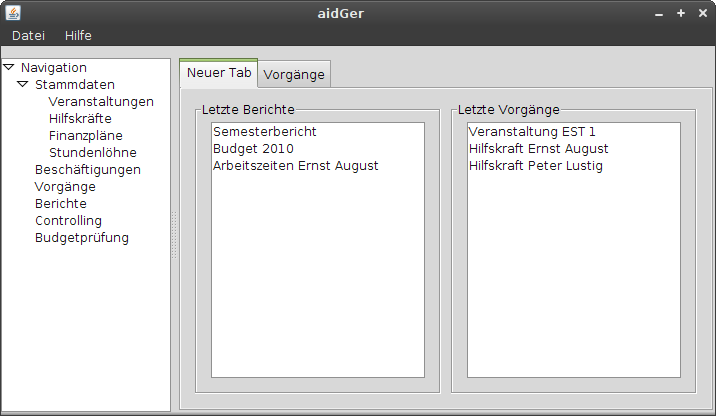
\includegraphics[scale=0.75]{mockup1} 
\par\end{center}

Das Hauptfenster ist in zwei Bereiche eingeteilt. Auf der linken Seite
befindet sich die Navigationsleiste, in der alle Funktionen angezeigt
werden und der Benutzer einfach zwischen ihnen wechseln kann. Auf
der rechten Seite befindet sich der Inhaltsbereich. Hier wird die
aktuell ausgewählte Funktion angezeigt. Im Hintergrund können zudem
noch weitere Funktionen offen sein. Diese befinden sich dann in weiteren
Tabs. Im Beispiel wäre der {}``Neue Tab'' der aktuell geöffnete
und {}``Vorgänge'' ein sich im Hintergrund befindlicher Tab.\\
 \\
 Die Navigationsleiste und der Inhaltsbereich sind durch eine
bewegliche, vertikale Leiste getrennt. Dadurch kann die Größe beider
Bereiche individuell angepasst werden.


\subsection{Verhalten bei Änderung der Fenstergröße\label{sub:Verhalten-bei-=00003D0000C4nderung}}

Bei einer Veränderung der Fenstergröße in der Breite wird nur der
Inhaltsbereich verändert um mehr Platz für Informationen/Formulare
zu bekommen. Die Navigationsleiste wird höchstens so breit wie das
breiteste Element in ihr.\\
 \\
 Sollte sich die Fenstergröße in der Höhe verändern, ändert sich
die Größe beider Elemente gleichmäßig.


\subsection{Verhalten bei Auswahl eines Elements in der Navigationsleiste\label{sub:Verhalten-bei-Auswahl}}

Wird vom Benutzer ein Element in der Navigationsleiste mit der linken
Maustaste ausgewählt, wird der aktuelle Inhalt des Inhaltsbereichs
verworfen und durch den Inhalt des neuen Elements ersetzt. \\
 Sollte der Benutzer jedoch die mittlere Maustaste benutzen um
das Element auszuwählen, wird ein neuer Reiter geöffnet und der Inhalt
des Elements in diesem neuen Reiter dargestellt. Der aktuelle Reiter
bleibt dabei vollständig erhalten, gerät jedoch in den Hintergrund
(ist also nicht mehr sichtbar).


\section{Navigationselemente\label{sec:Navigationselemente}}

%TODO: Alle Navigationselemente aufzählen


In der folgenden Gliederung der Navigationsleiste sind die obersten
Elemente die Hauptelemente und darunter folgende Sublisten die dementsprechenden
Menüs die aufklappen sobald man auf das Hauptelement klickt. Nur beim
Auswählen der Unterpunkte wird der Inhalt des Inhaltsbereiches verändert.
\begin{itemize}
\item Stammdatenverwaltung 
\begin{itemize}
\item Veranstaltungen 
\item Hilfskräfte 
\item Finanzpläne 
\item Stundenlöhne 
\end{itemize}

\item Beschäftigungen

\item Vorgänge 

\item Reports 

\item Controlling 

\item Budgetprüfung 

\end{itemize}

\section{Menüleiste\label{sec:Men=00003D0000FCleiste}}

Die Menüleiste befindet sich unter Windows und Linux unterhalb des
Fensterrahmens aber oberhalb der Navigationsleiste und des Inhaltsbereichs.
Unter Mac OS X befindet sie sich in einer Leiste unter dem oberen
Bildschirmrand. \\
 In der folgenden Gliederung dieser Menüleiste sind die obersten
Elemente die Hauptelemente und darunter folgende Sublisten die dementsprechenden
Menüs die aufklappen sobald man auf das Hauptelement klickt.
\begin{itemize}
\item Datei 

\begin{itemize}
\item Drucken 
\item Einstellungen 
\item $----------$ 
\item Beenden 
\end{itemize}
\item Hilfe 

\begin{itemize}
\item Hilfe 
\item Über 
\end{itemize}
\end{itemize}

\section{Stammdatenverwaltung}

Die GUI für die Stammdatenverwaltung wird hier am Beispiel der Veranstaltungen
gezeigt. Für die anderen Stammdaten ist diese ähnlich bis gleich.
Hauptunterschied sind dabei die dort dargestellten Daten und Formulare.


\subsection{Hauptanzeige}

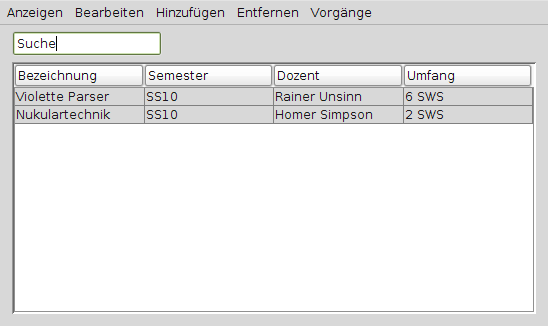
\includegraphics{MockupVeranstaltungen}

Nach einem Klick auf Stammdatenverwaltung $\rightarrow$ Veranstaltungen
wird die Hauptansicht der Stammdatenverwaltung angezeigt. Diese besteht
aus einer Toolbar am oberen Rand und einer tabellarischen Darstellung
aller vorhandenen Daten. Zudem gibt es dazwischen noch ein Suchfeld. 
Zu Beginn ist die Tabelle auf einige wichtige
Spalten beschränkt. Über ein Kontextmenü können jedoch alle verfügbaren
Daten in der Tabelle angezeigt werden um einen breiten Bildschirm
voll auszunützen. \\
Die Suche aktualisiert die Tabelle sobald der erste Buchstabe eingegeben wurde
automatisch und ohne das ein Knopf gedrückt werden muss.\\
In der Toolbar befinden sich die Buttons {}``Anzeigen'' zum
Anzeigen der Details des momentan ausgewählten Tabelleneintrags, {}``Bearbeiten''
um die ausgewählte Veranstaltung zu verändern, {}``Hinzufügen''
um eine neue Veranstaltung hinzuzufügen, {}``Entfernen'' um die
ausgewählte Veranstaltung zu entfernen und {}``Vorgänge'' um direkt
zu den Vorgängen der ausgewählten Veranstaltung zu springen. Um einen
Tabelleneintrag anzuzeigen kann auch ein Doppelklick auf ihn ausgeführt
werden. Per Entf-Taste kann ein Eintrag zudem entfernt werden.


\subsection{Anzeigen}

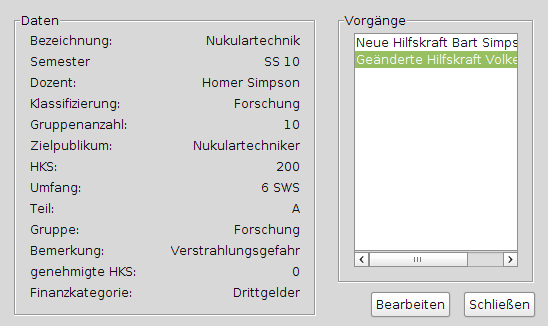
\includegraphics{MockupVeranstaltungenAnzeige}

Hier werden alle vorhandenen Daten zum ausgewählten Datensatz angezeigt.
Sollte beim Klick auf den {}``Anzeigen''-Button jedoch kein Eintrag
ausgewählt worden sein, so wird der Nutzer dadurch durch eine Fehlermeldung
hingewiesen. \\
 Die Anzeige gliedert sich in zwei Abschnitte. Im Linken werden
alle Daten angezeigt. Im Rechten wird die eingestellte Anzahl von
Vorgängen (\ref{sec:Programmeinstellungen}) zu diesem Datensatz angezeigt.
Durch einen Doppelklick auf einen Vorgang wird dieser angezeigt. \\
 Unterhalb dieser Abschnitte befinden sich noch zwei Buttons.
Der {}``Schließen''-Button dient hierbei zum Schließen des Fensters
und zurückkehren zur letzten Ansicht und der {}``Bearbeiten''-Button
um die Daten zu verändern.


\subsection{Bearbeiten}

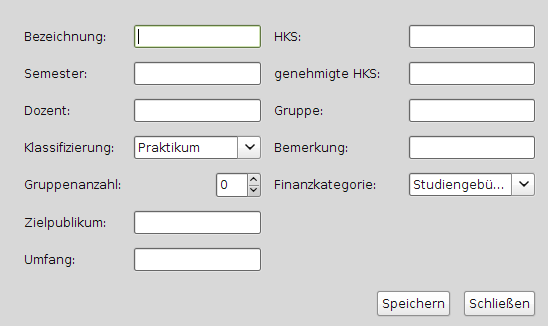
\includegraphics{MockupVeranstaltungenBearbeiten}

Diese Ansicht bietet die Möglichkeit alle Daten eines Datensatzes
zu verändern. Sollte dieser Dialog über die Hauptansicht aufgerufen
werden und kein Eintrag selektiert sein, so wird der Nutzer durch
eine Fehlermeldung darauf hingewiesen. \\
 Die Ansicht bietet eine Reihe von Eingabefeldern um die Daten
zu verändern. Unter diesen befinden sich zwei Buttons. Der {}``Speichern''-Button
speichert die neuen Daten in der Datenbank und schließt die Ansicht,
der {}``Abbrechen''-Button schließt sie ebenfalls, jedoch ohne die
Daten in der Datenbank zu speichern. \\
 Beim Speichern werden die eingetragenen Daten auf ihre Korrektheit
überprüft. Sollten sich in einem Eingabefeld inkorrekte Daten befinden
(zum Beispiel ein Name in einem Datumsfeld) so wird der Nutzer darauf
hingewiesen und kann die Daten erst speichern nachdem alle Daten korrekt
sind.


\subsection{Hinzufügen}

Die {}``Hinzufügen''-Ansicht ist prinzipiell dieselbe wie die {}``Bearbeiten''-Ansicht.
Einzigster Unterschied ist das sich hier noch keine Daten in den Eingabefeldern
befinden und das der {}``Speichern''-Button einen neuen Eintrag
in der Datenbank anlegt.


\subsection{Entfernen}

Beim Löschen wird der momentan ausgewählte Eintrag in der Tabelle
entfernt. Sollte kein Eintrag ausgewählt sein, so wird der Nutzer
durch eine Fehlermeldung darauf hingewiesen. \\
 Bevor der Eintrag gelöscht wird, wird der Nutzer gefragt ob er
diesen Vorgang wirklich durchführen will um das versehentliche Löschen
eines Eintrags zu verhindern.


\subsection{Vorgänge}

Hier wird eine Liste aller Vorgänge zu dem ausgewählten Datensatz
angezeigt. Sollte kein Datensatz ausgewählt sein, so wird der Nutzer
durch eine Fehlermeldung darauf hingewiesen. \\
 Durch einen Doppelklick auf einen Vorgang wird dieser angezeigt.

\section{Beschäftigungen}

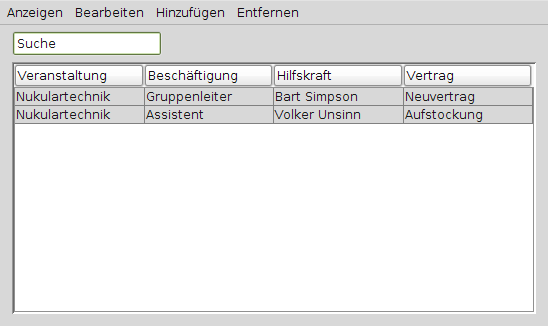
\includegraphics{MockupBuchungen.png}

Bei den Beschäftigungen wird die von der Stammdatenhauptansicht bekannte Form benutzt.
Das heisst das sich am oberen Rand eine Toolbar befindet in der es die Funktionen
``Anzeigen'', ``Bearbeiten'', ``Hinzufügen'' und ``Entfernen'' gibt. Darunter
befindet sich ein Eingabefeld das zur Suche in der Tabelle dient und letztendlich
die Tabelle in der die Daten dargestellt werden.\\
Die Suche aktualisiert die Tabelle sobald der erste Buchstabe eingegeben wurde
automatisch und benötigt keinen Suchknopf.\\

Die Ansichten zum Anzeigen, Bearbeiten, Hinzufügen und Entfernen sind größtenteils
Äquivalent zu ihren Gegenübern in der Stammdatenverwaltung. \\

\subsection{Anzeigen}

Die normale ``Anzeigen''-Ansicht der Stammdatenverwaltug wird noch um Verweise
auf die Hilfskraft und die Veranstaltung erweitert um schnell an wichtige Informationen
zu kommen. Zudem werden hier alle wichtigen Vertragsdetails angezeigt.

\subsection{Bearbeiten und Hinzufügen}

Hier können die Veranstaltungen und Hilfskräfte einfach per Combobox aus den bereits
vorhandenen ausgesucht werden sowie über Verweise auf die entsprechenden Ansichten
schnell hinzugefügt werden.

\section{Vorgänge}

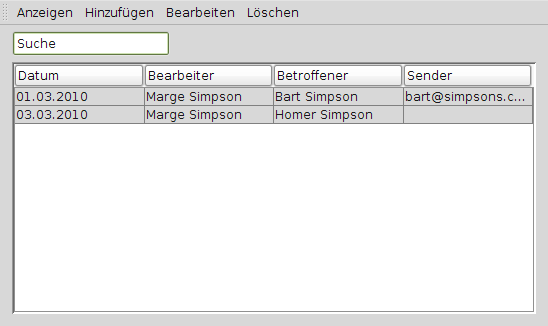
\includegraphics{MockupVorgaenge.png}

Die ``Vorgänge''-Ansicht ist ebenfalls ähnlich wie die Stammdatenhauptansicht aufgebaut.
Am oberen Rand befindet sich eine Toolbar mit 4 Knöpfen ``Anzeigen'', ``Bearbeiten'',
``Hinzufügen'' und ``Entfernen''. Darunter befindet sich ein Suchfeld und letztendlich
die Tabelle mit allen Vorgängen, standardmäßig sortiert nach dem Zeitpunkt des
Vorgangs.\\
Wird in das Suchfeld etwas hineingeschrieben, wird sofort die Tabelle darunter
aktualisiert und es werden nur noch Vorgänge angezeigt, die in einem ihrer Felder
mit dem Suchwort beginnen.\\

Die Ansichten zum Anzeigen, Bearbeiten, Hinzufügen oder Entfernen entsprechen
größtenteils ihren Equivalenten aus der Stammdatenverwaltung. Deshalb werden
im Folgenden nur die Unterschiede aufgezeigt.

\subsection{Anzeigen}

In der ``Anzeigen''-Ansicht befinden sich zusätzlich Verweise um auf die im
Vorgang betroffenen Stammdaten einfach zugreifen können. Ein Klick auf einen
dieser Verweise öffnet dann zum Beispiel die Anzeige der Hilfskraftdetails in 
einem neuen Tab.

\subsection{Bearbeiten und Hinzufügen}

Hier sind die einzigsten Unterschiede das Verweise auf Stammdaten aus Comboboxen
ausgesucht werden können um schnellstmöglichst auf diese Zugreifen zu können.

\section{Reports}

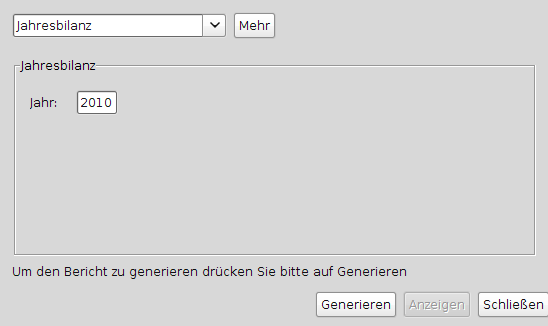
\includegraphics{MockupReports.png}

Die möglichen Berichte die generiert werden können, werden hier in einem Drop-Down-Feld
angezeigt. Über den ``Mehr''-Button kann man sich die darunter befindlichen
Einstellungsmöglichkeiten einblenden lassen (davor sind diese nicht sichtbar).
Nach dem Ausfüllen der Felder kann dann über den ``Generieren''-Button der Bericht
generiert werden. Dieser wird dann je nach Einstellung automatisch geöffnet oder
kann dann durch einen Klick auf ``Anzeigen'' angezeigt werden. 
Der ``Schließen''-Button schließt die ``Reports''-Ansicht und kehrt zur vorherigen 
Ansicht bzw. der ``Neuer Tab''-Ansicht zurück.

\section{Controlling}

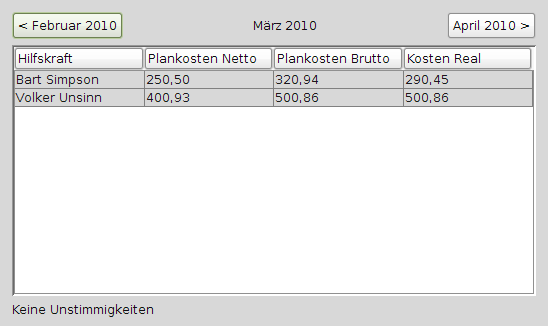
\includegraphics{MockupControlling.png}

Die ``Controlling''-Ansicht ist zweigeteilt. Oben befindet sich die Monatskontrollleiste.
Mit ihr kann man zwischen den Monaten hin- und hernavigieren um den gewünschten Monat
zu erreichen. Darunter werden für den jeweiligen Monat die entsprechenden 
geplanten Kosten für alle Hilfskräfte einzeln in tabellarischer Form aufgelistet.

\section{Budgetprüfung}

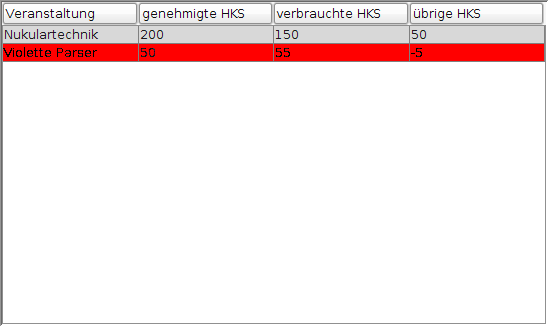
\includegraphics{MockupBudgetPruefung.png}

Unter ``Budgetprüfung'' werden alle Veranstaltungen in Tabellenform aufgelistet.
Dabei wird jedoch nur die Anzahl der genehmigten HKS, der schon verbrauchten und
der noch übrig gebliebenen HKS angezeigt. Veranstaltungen die schon mehr HKS 
verbraucht haben als eigentlich genehmigt wurden werden zudem rot hinterlegt.
So ist sofort ersichtlich wo das Budget schon verbraucht ist und wo noch nicht.

\section{Drucken\label{sec:Drucken}}

Zum Drucken wird der von Java bereitgestellte Druckdialog verwendet. Dieser erlaubt
zum Beispiel die Einstellung des Druckers und der Anzahl der Kopien.

\section{Programmeinstellungen\label{sec:Programmeinstellungen}}

%TODO: Einstellung für Anzahl von Vorgängen bei Anzeigen hinzufügen


\begin{center}
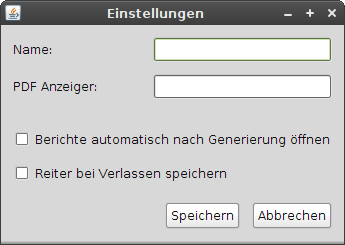
\includegraphics{MockupSettings} 
\par\end{center}

Das Einstellungsfenster ist ein modaler Dialog, der über keine Menüleiste
verfügt. Ganz unten verfügt er über zwei Buttons. Über den Abbrechen-Button
schließt sich das Fenster ohne die Einstellungen zu speichern. Mit
Hilfe des Speichern-Buttons werden die Einstellungen vor dem Schließen
noch gespeichert. \\
 Es befinden sich folgende Einstellungsmöglichkeiten im Fenster: 
\begin{itemize}
\item \textbf{Name} \\
 Der hier eingetragene Name wird zur Kennzeichnung der Vorgänge
benutzt. Das bedeutet das Vorgänge unter diesem Namen ins System eingetragen
werden. 
\item \textbf{PDF-Anzeiger} \\
 Pfad zu einem Programm das PDFs anzeigen kann. Der Pfad zur PDF-Datei
wird hierbei als Argument für das Programm übergeben. 
\item \textbf{Anzahl der Vorgänge}\\
Die Anzahl der Vorgänge die in Detailansichten wie zum Beispiel bei den Stammdaten
von Hilfskräften angezeigt werden sollen.
\item \textbf{Berichte automatisch nach Generierung öffnen} \\
 Wenn aktiviert öffnen sich Berichte direkt nach ihrer Generierung
automatisch im unter {}``PDF-Anzeiger'' angegeben PDF-Programm oder
in dem standardmäßig verwendeten Programm. 
\item \textbf{Reiter bei Verlassen speichern} \\
 Wenn aktiviert werden alle geöffneten Reiter gespeichert und
beim nächsten Aufruf des Programms wieder geöffnet um dem Nutzer die
Weiterführung seiner Arbeit zu erleichtern. 
\end{itemize}

\section{Über-Fenster\label{sec:=00003D0000DCber-Fenster}}

Das Über-Fenster enthält den Programmnamen und die Programmversion
(sowie das zugehörige Veröffentlichungsdatum), die Namen der Entwickler
und einen Verweis auf die Projektwebsite.


\chapter{Anwendungsfälle\label{cha:Anwendungsf=0000E4lle}}

In diesem Kapitel sollen die wichtigsten Anwendungsfälle des Systems
dargestellt werden.


\section{Use-Case-Diagramm\label{sec:Use-Case-Diagramm}}

..

\setlength{\tabcolsep}{8pt} \renewcommand{\arraystretch}{1.5}


\section{Anwendungsfall X}

\begin{center}
\begin{longtable}{|>{\raggedright}p{3.5cm}|>{\raggedright}p{10.5cm}|}
\hline 
\multicolumn{2}{|c|}{\textbf{Name}}\tabularnewline
\hline
\hline 
\textbf{Vorbedingung:} & \tabularnewline
\hline 
\textbf{Regulärer Ablauf:} & \begin{enumerate}
\item ..
\item ..
\end{enumerate}
\tabularnewline
\hline 
\textbf{Nachbedingung:} & \tabularnewline
\hline 
\textbf{Alternativer Ablauf:} & \tabularnewline
\hline 
\textbf{Nachbedingung im Sonderfall:} & \tabularnewline
\hline
\end{longtable}
\par\end{center}


\section{Stammdaten hinzufügen}

\begin{center}
\begin{longtable}{|>{\raggedright}p{3.5cm}|>{\raggedright}p{10.5cm}|}
\hline 
\multicolumn{2}{|c|}{\textbf{Stammdaten hinzufügen}}\tabularnewline
\hline
\hline 
\textbf{Vorbedingung:} & Benutzer befindet sich in der Stammdatenverwaltung.\tabularnewline
\hline 
\textbf{Regulärer Ablauf:} & \begin{enumerate}
\item Benutzer klickt auf den Button ,,Hinzufügen{}``
\item Es öffnet sich das ,,Hinzufügen{}``-Popup
\item Benutzer gibt die erforderlichen Daten ein
\item Benutzer klickt auf den Button ,,OK{}``
\item Das Popup schließt sich
\end{enumerate}
\tabularnewline
\hline 
\textbf{Nachbedingung:} & Die neuen Stammdaten wurden hinzugefügt und der Benutzer befindet
sich wieder in der Stammdatenverwaltung.\tabularnewline
\hline 
\textbf{Alternativer Ablauf:} & \begin{enumerate}
\item Benutzer gibt erforderliche Daten falsch ein

\begin{enumerate}
\item Fehlerhafte Felder werden markiert
\item Meldung erscheint, dass markierte Felder korrigiert werden müssen
\item Benutzer korrigiert die fehlerhaften Felder
\item Benutzer klickt auf den Button ,,OK{}``
\item Das Popup schließt sich
\end{enumerate}
\item Benutzer klickt auf den Button ,,Abbrechen{}``

\begin{enumerate}
\item Das Popup schließt sich
\end{enumerate}
\end{enumerate}
\tabularnewline
\hline 
\textbf{Nachbedingung im Sonderfall:} & \begin{enumerate}
\item Die neuen (fehlerfreien) Stammdaten wurden hinzugefügt und der Benutzer
befindet sich wieder in der Stammdatenverwaltung
\item Es wurden keine Stammdaten hinzugefügt und der Benutzer befindet sich
wieder in der Stammdatenverwaltung
\end{enumerate}
\tabularnewline
\hline
\end{longtable}
\par\end{center}


\section{Stammdaten bearbeiten}

\begin{center}
\begin{longtable}{|>{\raggedright}p{3.5cm}|>{\raggedright}p{10.5cm}|}
\hline 
\multicolumn{2}{|c|}{\textbf{Stammdaten bearbeiten}}\tabularnewline
\hline
\hline 
\textbf{Vorbedingung:} & Benutzer befindet sich in der Stammdatenverwaltung.\tabularnewline
\hline 
\textbf{Regulärer Ablauf:} & \begin{enumerate}
\item Benutzer markiert ein Datum
\item Benutzer klickt auf den Button ,,Bearbeiten{}``
\item Das ,,Bearbeiten{}``-Popup öffnet sich
\item Benutzer ändert die gewünschten Daten
\item Benutzer klickt auf ,,OK{}``
\item Das Popup schließt sich
\end{enumerate}
\tabularnewline
\hline 
\textbf{Nachbedingung:} & Das Datum wurde geändert und der Benutzer befindet sich wieder in
der Stammdatenverwaltung.\tabularnewline
\hline 
\textbf{Alternativer Ablauf:} & \begin{enumerate}
\item Benutzer hat kein Datum markiert und klickt auf ,,Bearbeiten{}``

\begin{enumerate}
\item Fehler wird in der Hinweisleiste angezeigt
\end{enumerate}
\item Benutzer gibt erforderliche Daten falsch ein

\begin{enumerate}
\item Fehlerhafte Felder werden markiert
\item Meldung erscheint, dass markierte Felder korrigiert werden müssen
\item Benutzer korrigiert die fehlerhaften Felder
\item Benutzer klickt auf den Button ,,OK{}``
\item Das Popup schließt sich
\end{enumerate}
\item Benutzer klickt auf den Button ,,Abbrechen{}``

\begin{enumerate}
\item Das Popup schließt sich
\end{enumerate}
\end{enumerate}
\tabularnewline
\hline 
\textbf{Nachbedingung im Sonderfall:} & \begin{enumerate}
\item Es wurde kein Datum verändert und der Benutzer befindet sich immer
noch in der Stammdatenverwaltung
\item Das Datum wurde verändert und der Benutzer befindet sich wieder in
der Stammdatenverwaltung
\item Es wurde kein Datum verändert und der Benutzer befindet sich wieder
in der Stammdatenverwaltung
\end{enumerate}
\tabularnewline
\hline
\end{longtable}
\par\end{center}


\section{Stammdaten löschen}

\begin{center}
\begin{longtable}{|>{\raggedright}p{3.5cm}|>{\raggedright}p{10.5cm}|}
\hline 
\multicolumn{2}{|c|}{\textbf{Stammdaten löschen}}\tabularnewline
\hline
\hline 
\textbf{Vorbedingung:} & Benutzer befindet sich in der Stammdatenverwaltung\tabularnewline
\hline 
\textbf{Regulärer Ablauf:} & \begin{enumerate}
\item Benutzer markiert ein Datum
\item Benutzer klickt auf den Button ,,Löschen{}``
\item Das ,,Bestätigungs{}``-Popup öffnet sich
\item Benutzer klickt auf den Button ,,Ja{}``
\item Das Popup schließt sich
\end{enumerate}
\tabularnewline
\hline 
\textbf{Nachbedingung:} & Das Datum wurde gelöscht und der Benutzer befindet sich weiterhin
in der Stammdatenverwaltung.\tabularnewline
\hline 
\textbf{Alternativer Ablauf:} & \begin{enumerate}
\item Das Datum wird referenziert

\begin{enumerate}
\item Fehler wird in der Hinweisleiste angezeigt
\end{enumerate}
\item Der Benutzer klickt in dem ,,Bestätigungs{}``-Popup auf ,,Nein{}``

\begin{enumerate}
\item Das Popup schließt sich
\end{enumerate}
\end{enumerate}
\tabularnewline
\hline 
\textbf{Nachbedingung im Sonderfall:} & \begin{enumerate}
\item Das Datum wurde nicht gelöscht und der Benutzer befindet sich weiterhin
in der Stammdatenverwaltung
\item Das Datum wurde nicht gelöscht und der Benutzer befindet sich weiterhin
in der Stammdatenverwaltung
\end{enumerate}
\tabularnewline
\hline
\end{longtable}
\par\end{center}


\chapter{Anhang\label{cha:Anhang}}


\section{Begriffslexikon\label{sec:Begriffslexikon}}


\paragraph*{Aufstockung}

Erweiterung eines Vertrages, so dass die Hilfskraft für mehrere Veranstaltungen,
aus verschiedenen Fonds finanziert, verwendet werden kann.


\paragraph*{Aufwendung}

Durch das Buchen von Beschäftigungen entstandener Aufwand.


\paragraph*{Beschäftigung}

Eine Einstellung einer Hilfskraft über einen bestimmten Zeitraum für
eine oder mehrere Veranstaltungen.


\paragraph*{Bericht}

Ein PDF-Dokument zum Überblick über alle im System eingetragenen Informationen.


\paragraph*{Bilanz}

Aufstellung der Plankosten für Veranstaltungen für jede Gruppe.


\paragraph*{Buchung}

Erstellung einer Beschäftigung für eine Hilfskraft.


\paragraph*{Budget}

Kennzahl der verfügbaren HKS einer Veranstaltung.


\paragraph*{Budgetprüfung}

Informationen über das gebuchte und eingeplante Budget erlangen.


\paragraph*{Controlling}

Die Überprüfung und der Vergleich von Abrechnungen auf deren Korrektheit.


\paragraph*{Diff-Tabelle}

Ein Monatsauzug aller Hilfskräfte.


\paragraph*{Dozent}

Eine Person, die eine Veranstaltung verwaltet.


\paragraph*{Finanzkategorie}

Einstufung der Beschäftigung nach Kategorien aufgrund unterschiedlicher
Vergütungen.


\paragraph*{Finanzplan}

Zuordnung von Finanzkategorien zu deren Plankostenhaushalt pro Jahr.


\paragraph*{Fonds}

Verfügbare Kapitalanlagen.


\paragraph*{Gruppe}

Zuordnung der Veranstaltung zu einem Themengebiet oder Studiengang.


\paragraph*{Handicap}

Ein Multiplikator, welcher, je nach Qualifikation der Hilfskräfte,
dafür vorgesehen war, das Gehalt anzupassen.


\paragraph*{Haushalt}

Einnahmen und Ausgaben der Universität.


\paragraph*{Hilfskraft}

Eine Person, welche am Institutsverbund Informatik eingestellt ist.


\paragraph*{HKS}

Hilfskraftstunden


\paragraph*{Kostenstelle}

Klassifikation des Fonds in eine Ziffer.


\paragraph*{Monatsauszug}

Ein Auflistung aller Plankosten der Hilfskräfte.


\paragraph*{Plankosten}

Im System für einen Zeitraum hinterlegte und daher geplante Kosten.


\paragraph*{Plankostenhaushalt}

Plankosten, die einseits aus dem Haushalt, aber auch aus Studiengebühren
finanziert werden.


\paragraph*{Protokoll}

Eine Tabelle, die alle getätigten Vorgänge für einen Tag enthält.


\paragraph*{Qualifikation}

Die Qualifikation einer Hilfskraft ist entweder geprüft, ungeprüft
oder ein Bachelor-Abschluss.


\paragraph*{Stammdaten}

Wesentliche Daten, die bei der Hilfskräfteverwaltung hinterlegt werden
müssen.


\paragraph*{Stundenlohn}

Der Gehalt, den eine Hilfskraft, pro Stunde erhält.


\paragraph*{Tätigkeitsnachweis}

Ein offizielles Schreiben, welches Informationen über Hilfskräfte
und deren Vorgänge enthält.


\paragraph*{Teil}

Aufspaltung einer Veranstaltung nach mehreren Zielgruppen.


\paragraph*{Ticket}

Ein Vorgang, der ausschließlich über das Ticket-System verwaltet wird.


\paragraph*{Übungsgruppe}

Eine Versammlung von Studenten, die von einer Hilfskraft betreut wird.


\paragraph*{Umfang}

Angabe der benötigten Semesterwochenstunden für eine Veranstaltung.


\paragraph*{Uni-Budget}

Siehe Haushalt.


\paragraph*{Veranstaltung}

Eine Beschäftigung (Forschung, Praktikum, Lehre), für die ein Dozent
verantwortlich ist.


\paragraph*{Vertrag}

Eine schriftliche Vereinbarung zwischen der Hilfskraft und dem Institutsverbund.
Kann aus mehreren Beschäftigungen bestehen, falls diese aus dem gleichen
Fonds finanziert werden.


\paragraph*{Vorgang}

Ein Prozess, der beim Verwalten von Hilfskräften anfällt.


\section{Versionshistorie\label{sec:Versionshistorie}}


\subsection*{Version 0.2 (08.03.2010)}
\begin{itemize}
\item Konkretisierung der Anforderungen
\item Verfeinerungen in Kapitel \ref{cha:Allgemeine-Beschreibung}, \ref{cha:Anforderungen}
und \ref{cha:Benutzeroberfl=0000E4che}
\item Erstellung des Kapitels \ref{cha:Anwendungsf=0000E4lle}
\item Begriffslexikon hinzugefügt und erweitert
\end{itemize}

\subsection*{Version 0.1.1 (07.03.2010)}
\begin{itemize}
\item Sammeln von Anforderungen und Auflistung der Anforderungen in Kapitel
\ref{cha:Anforderungen}
\item Erste Mockups und Erklärungen für Kapitel \ref{cha:Benutzeroberfl=0000E4che}
\item Erstellung des Begriffslexikons
\end{itemize}

\subsection*{Version 0.1 (06.03.2010)}
\begin{itemize}
\item Erstellung der Grundstruktur dieses Dokuments
\item Erstellung des Kapitels \ref{cha:Einleitung} und \ref{cha:Allgemeine-Beschreibung}
\end{itemize}

\end{document}
